\pgfsetplotmarksize{0pt}
\begin{figure}
 \centering
 \caption{\label{CBCvsMSTAV-d05}CBCvsMSTAV-d05},
 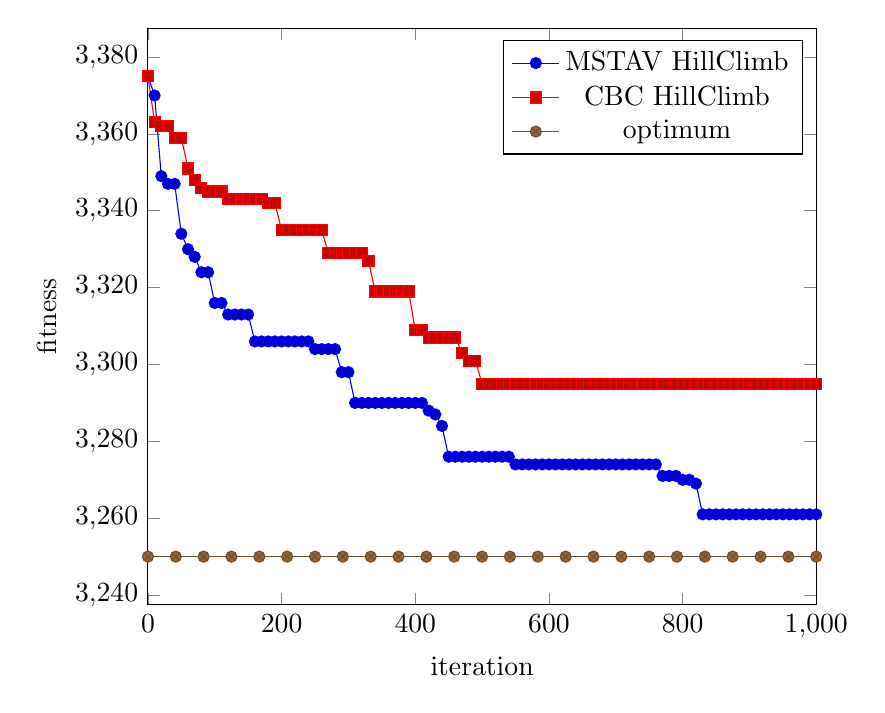
\begin{tikzpicture}
 \begin{axis}[
   width=0.7\textwidth,
   scale only axis,
   xlabel=iteration,
   ylabel=fitness,
   xmin=0,xmax=1000,
   domain=0:1000]
   \addplot coordinates {
     (0,3375)
     (10,3370)
     (20,3349)
     (30,3347)
     (40,3347)
     (50,3334)
     (60,3330)
     (70,3328)
     (80,3324)
     (90,3324)
     (100,3316)
     (110,3316)
     (120,3313)
     (130,3313)
     (140,3313)
     (150,3313)
     (160,3306)
     (170,3306)
     (180,3306)
     (190,3306)
     (200,3306)
     (210,3306)
     (220,3306)
     (230,3306)
     (240,3306)
     (250,3304)
     (260,3304)
     (270,3304)
     (280,3304)
     (290,3298)
     (300,3298)
     (310,3290)
     (320,3290)
     (330,3290)
     (340,3290)
     (350,3290)
     (360,3290)
     (370,3290)
     (380,3290)
     (390,3290)
     (400,3290)
     (410,3290)
     (420,3288)
     (430,3287)
     (440,3284)
     (450,3276)
     (460,3276)
     (470,3276)
     (480,3276)
     (490,3276)
     (500,3276)
     (510,3276)
     (520,3276)
     (530,3276)
     (540,3276)
     (550,3274)
     (560,3274)
     (570,3274)
     (580,3274)
     (590,3274)
     (600,3274)
     (610,3274)
     (620,3274)
     (630,3274)
     (640,3274)
     (650,3274)
     (660,3274)
     (670,3274)
     (680,3274)
     (690,3274)
     (700,3274)
     (710,3274)
     (720,3274)
     (730,3274)
     (740,3274)
     (750,3274)
     (760,3274)
     (770,3271)
     (780,3271)
     (790,3271)
     (800,3270)
     (810,3270)
     (820,3269)
     (830,3261)
     (840,3261)
     (850,3261)
     (860,3261)
     (870,3261)
     (880,3261)
     (890,3261)
     (900,3261)
     (910,3261)
     (920,3261)
     (930,3261)
     (940,3261)
     (950,3261)
     (960,3261)
     (970,3261)
     (980,3261)
     (990,3261)
     (1000,3261)
   };
   \addlegendentry{MSTAV HillClimb}
   \addplot coordinates {
     (0,3375)
     (10,3363)
     (20,3362)
     (30,3362)
     (40,3359)
     (50,3359)
     (60,3351)
     (70,3348)
     (80,3346)
     (90,3345)
     (100,3345)
     (110,3345)
     (120,3343)
     (130,3343)
     (140,3343)
     (150,3343)
     (160,3343)
     (170,3343)
     (180,3342)
     (190,3342)
     (200,3335)
     (210,3335)
     (220,3335)
     (230,3335)
     (240,3335)
     (250,3335)
     (260,3335)
     (270,3329)
     (280,3329)
     (290,3329)
     (300,3329)
     (310,3329)
     (320,3329)
     (330,3327)
     (340,3319)
     (350,3319)
     (360,3319)
     (370,3319)
     (380,3319)
     (390,3319)
     (400,3309)
     (410,3309)
     (420,3307)
     (430,3307)
     (440,3307)
     (450,3307)
     (460,3307)
     (470,3303)
     (480,3301)
     (490,3301)
     (500,3295)
     (510,3295)
     (520,3295)
     (530,3295)
     (540,3295)
     (550,3295)
     (560,3295)
     (570,3295)
     (580,3295)
     (590,3295)
     (600,3295)
     (610,3295)
     (620,3295)
     (630,3295)
     (640,3295)
     (650,3295)
     (660,3295)
     (670,3295)
     (680,3295)
     (690,3295)
     (700,3295)
     (710,3295)
     (720,3295)
     (730,3295)
     (740,3295)
     (750,3295)
     (760,3295)
     (770,3295)
     (780,3295)
     (790,3295)
     (800,3295)
     (810,3295)
     (820,3295)
     (830,3295)
     (840,3295)
     (850,3295)
     (860,3295)
     (870,3295)
     (880,3295)
     (890,3295)
     (900,3295)
     (910,3295)
     (920,3295)
     (930,3295)
     (940,3295)
     (950,3295)
     (960,3295)
     (970,3295)
     (980,3295)
     (990,3295)
     (1000,3295)
   };
   \addlegendentry{CBC HillClimb}
   \addplot {3250.000000};
   \addlegendentry{optimum}
 \end{axis}
 \end{tikzpicture}
\end{figure}
